\documentclass[11pt, a4paper]{article}
\usepackage{amsmath,graphicx}
\usepackage{cite}
\usepackage{amsthm,amssymb,amsfonts}
\usepackage{textcomp}
\usepackage{bm}
\usepackage{algorithm}    
\usepackage{algorithmic}
\usepackage{booktabs}
\usepackage{enumerate}
\usepackage{extarrows}
\usepackage[colorlinks]{hyperref}
\usepackage{listings}
\usepackage{xcolor}


\setlength{\textwidth}{6.3in}%%
\setlength{\textheight}{9.8in}%%
\setlength{\topmargin}{0pt}%%
\setlength{\headsep}{-0.5in}%%
\setlength{\headheight}{0pt}%%
\setlength{\oddsidemargin}{0pt}%%
\setlength{\evensidemargin}{0pt}%%
\setlength{\parindent}{3.5ex}%%
\setlength{\parskip}{0pt}%%

\definecolor{myred}{rgb}{0.7,0.2,0.1}

\begin{document}

\title{\textbf{Machine Learning, Spring 2019}\\Homework 1}
\date{Wang Yuzhen\\2018E8018461008}
\author{}
\maketitle

\section{Preliminaries}
The weight update rule $\mathbf{w}(t+1)=\mathbf{w}(t) + y(t)\mathbf{x}(t)$ has the nice interpretation that it move in the direction of classifying $\mathbf{x}(t) $ correctly.
\begin{enumerate}[(a)]
\item Show that $y(t)\mathbf{w}^T(t)\mathbf{x}(t)<0$. [\textit{Hint}: $\mathbf{x}(t)$ is misclassified by $\mathbf{w}(t)$.] (5 points)


\item Show that $y(t)\mathbf{w}^T(t+1)\mathbf{x}(t)>y(t)\mathbf{w}^T(t)\mathbf{x}(t)$. [\textit{Hint}: Use update rule.] (5 points)

\item As far as classifying $\mathbf{x}(t)$ is concerned, argue that the move from $\mathbf{w}(t)$ to $\mathbf{w}(t+1)$ is a move `in the right direction'. (5 points)

\end{enumerate}
Solution================================================
\begin{enumerate}[(a)]
	\item 
    When
	$\mathbf{x}(t)$ is misclassified by $\mathbf{w}(t)$\\
	y=-1 but  $\mathbf{w}^T(t)\mathbf{x}(t)>0$;\\
	y=1 but  $\mathbf{w}^T(t)\mathbf{x}(t)<0$;\\
    one equation can written as $y(t)\mathbf{w}^T(t)\mathbf{x}(t)<0$.
	
	\item $y(t)\mathbf{w}^T(t+1)\mathbf{x}(t)\\=y(t) [\mathbf{w}^T(t)+y(t)\mathbf{x}(t)]  \mathbf{x}(t)\\
		=y(t)\mathbf{w}^T(t)\mathbf{x}(t) +y^{2}||x ||^{2}\\
		>y(t)\mathbf{w}^T(t)\mathbf{x}(t)$. 
	
	\item $||\mathbf{w}(t+1)|| ^{2}\\
	=||\mathbf{w}(t)+ y^{t} \mathbf{x}(t)||^{2}\\
	= ||\mathbf{w}(t)||^{2} +y^{2}||x ||^{2} + 2\mathbf{w}(t) y^{t} \mathbf{x}(t)\\
	<||\mathbf{w}(t)||^{2}+||x(t)||^{2}
	$\\
	If $y(t)\mathbf{w}^T(t)\mathbf{x}(t)<0$,
	use the weight update rule $\mathbf{w}(t+1)=\mathbf{w}(t) + y(t)\mathbf{x}(t)$.
	 
	After finte steps, the move from $\mathbf{w}(t)$ to $\mathbf{w}(t+1)$ is a move `in the right direction'.\\
=========================================================
	\end{enumerate}





\section{Understanding the law of large numbers}
The Hoeffding Inequality is one form of the \textit{law of large numbers}. One of the simple forms of that law is the \textit{Chebyshev Inequality}, which you will prove here.
\begin{enumerate}[(a)]
	\item If $t$ is a non-negative random variable, prove that for any $\alpha>0$, $\mathbb{P}[t\ge \alpha]\le \mathbb{E}(t)/\alpha.$ (5 points)
	\item If $u$ is any random variable with mean $\mu$ and variance $\sigma^2$, prove that for any $\alpha>0$, $\mathbb{P}[(u-\mu)^2\ge \alpha]\le \frac{\sigma^2}{\alpha}.$ (5 points)
	\item If $u_1,\ldots,u_N$ are iid random variables, each with mean $\mu$ and variance $\sigma^2$, and $u=\frac{1}{N}\sum_{n=1}^N u_n$, prove that for any $\alpha >0 $,
	\[
	\mathbb{P}[(u-\mu)^2\ge \alpha ]\le \frac{\sigma^2}{N\alpha}\,.
	\]
(10 points)
\end{enumerate}


Solution================================================
\begin{enumerate}[(a)]
	\item 
	$\mathbb{P}[t> \alpha] =\mathbb{E}[\mathbb{L}[t> \alpha]]
	=\mathbb{E}[t / \alpha] 
	=\mathbb{E}(t)/ \alpha $
	
	\item $\mathbb{P}[t\ge \alpha]\le \mathbb{E}(t)/\alpha,$\\
		  $ \mathbb{E}((u-\mu)^2)= \sigma^{2}$\\
		  $\mathbb{P}[(u-\mu)^2\ge \alpha]\le \frac{\sigma^2}{\alpha}.$

		  
	
	\item $Var[\frac{1}{N}\sum_{n=1}^N u_n]=\frac{1}{N^{2}} [Var[u_1] +......+Var[u_n]]\\
	    =\frac{\sigma^2}{N}$\\
		And, $\mathbb{P}[t\ge \alpha]\le \mathbb{E}(t)/\alpha,$\\
		Then \\
		\[
	    \mathbb{P}[(u-\mu)^2\ge \alpha ]\le \frac{\sigma^2}{N\alpha}\,.
		\]\\
		=========================================================
	\end{enumerate}






\section{Probability and independence}
Consider a sample of 10 marbles drawn independently from a bin that holds red and green marbles. The probability of a red marble is $\mu$. For $\mu= 0.05, \mu = 0.5$, and $\mu=0.8$, compute the probability of getting no red marbles ($v=0$) in the followig cases.
\begin{enumerate}[(a)]
	\item We draw only one such sample. Compute the probability that $v=0$. (5 points)
	\item We draw 1000 independent samples. Compute the probability that (at least) one of the samples has $v=0$. (5 points)
	\item Repeat (b) for 1000000 independent samples.  (10 points)
\end{enumerate}



Solution================================================
\begin{enumerate}[(a)]
	\item  $P_{0}=(1-u)^{10}$\\
	$ \quad [0.05]  \quad  (1-0.05)^{10} =0.5987\\
	 \qquad  \qquad [0.5] \quad(1-0.5)^{10}= 9.7656e-04\\
	  \qquad \qquad  [0.8]\quad (1-0.8)^{10}=.0240e-07$\\
	  \item $P_{1}=1-(1-P_{0})^{1000} $\\
	   \item $P_{1}=1-(1-P_{0})^{1000000} $\\
	=========================================================
	\end{enumerate}




\section{Two learning algorithms}
We are given a data set $\mathcal{D}$ of 25 training examples from an unknown target target
function $f : \mathcal{X} \rightarrow \mathcal{Y},$ where $\mathcal{X}=\mathbb{R}$ and $\mathcal{Y}=\{-1,+1\} .$ To learn $f,$ we use
a simple hypothesis set $\mathcal{H}=\left\{h_{1}, h_{2}\right\}$ where $h_{1}$ is the constant $+1$ function
and $h_{2}$ is the constant $-1$.

We consider two learning algorithms, S (smart) and C (crazy). S chooses the hypothesis that agrees the most with $\mathcal{D}$ and $C$ chooses the other hypothesis deliberately. Let us see how these algorithms perform out of sample from the deterministic and probabilistic points of view. Assume in the probabilistic view that there is a probability distribution on $\mathcal{X},$ and let $\mathbb{P}[f(\mathbf{x})=+1]=p $
\begin{enumerate}[(a)]
\item Can S produce a hypothesis that is guaranteed to perform better than random on any point outside $\mathcal{D}$? (5 points)

\item Assume for the rest of the exercise that all the examples in $\mathcal{D}$ have $y_{n}=+1 .$ Is it possible that the hypothesis that $C$ produces turns out to be better than the hypothesis that S produces? (5 points)

\item If $p=0.9$, what is the probability that S will produce a better hypothesis than $C$? (5 points)

\item  Is there any value of $p$ for which it is more likely than not that $C$ will produce a better hypothesis than $S$? (5 points)
\end{enumerate}

Solution================================================
\begin{enumerate}[(a)]
	\item  No, it can't.
	\item  Yes. It is possible that the hypothesis that $C$ produces turns out to be better than the hypothesis that S produces.   We don't know performance on any point outside.
    \item  $P(0.9>0.1)=1$
	\item  $If \quad P(p>1-p) \quad is \quad,possible, p<0.5$
=========================================================
	\end{enumerate}



\section{Learning a target function}

Consider a Boolean target function over a three-dimensional input space $\mathcal{X} = \{0,1\}^3$. We are given a data set $\mathcal{D}$ of five examples represented in the table below. We denote the binary output by o/$\bullet$ for visual clarity, where $y_n = f(\mathbf{x}_n)$ for $n = 1,2,3,4,5$. (Please refer to $P28-29$ of "Learning from data" for more details of the problem)

Solution================================================
\begin{figure}[h]
	\centering
	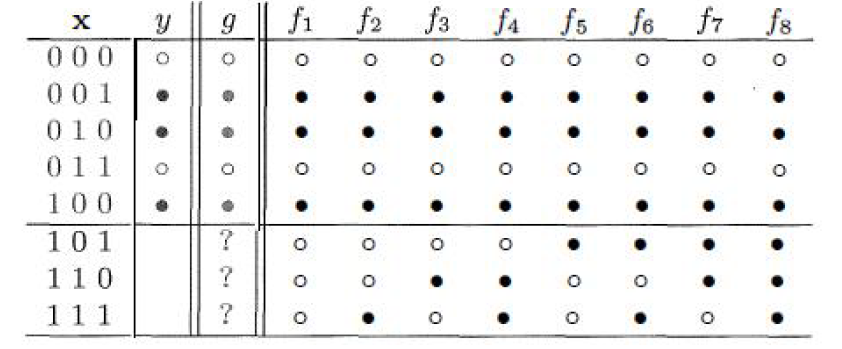
\includegraphics[width=0.4\linewidth]{1_8.png}
	\caption{Learning a target function}
	\label{fig:2}
\end{figure}
\begin{enumerate}[(a)]
	\item 
	a \quad all three points  \quad f8 \quad  two of them \quad f4,f6,f7\quad  one of them\quad f2,f3,f5 \quad
	
	\item b \quad all three points  \quad f1 \quad  two of them \quad f2,f3,f5\quad  one of them\quad f4,f6,f7 \quad

	\item c \quad all three points  \quad f2 \quad  two of them \quad f1,f4,f6\quad  one of them\quad f3,f5,f8 \quad
		
	\item d \quad all three points  \quad f7 \quad  two of them \quad f3,f5,f8\quad  one of them\quad f1,f4,f6 \quad
	
	=========================================================
	\end{enumerate}


\end{document}